\section{Il Cerchio}\label{subsec:the:circle}

Ricordiamo che l'equazione per un cerchio con centro in $(h,k)$ e raggio $r>0$ è la seguente: 

\begin{equation} \label{cerchio:equazione}
(x-h)^2+(y-k)^2=r^2
\end{equation}

\subsection{Esercizi}

\begin{enumerate}

\item  \label{circ_00}
% https://math.libretexts.org/
Write an equation of the circle centered at $(8 , -10)$ with radius $8$.
\rightline{ (Soluzione a pagina \pageref{circs_00} )}

\vspace{1cm}
\hrule
\vspace{1cm}


\item  \label{circ_01}

State the center and radius of the circle graphed below and construct the equation for it.

\begin{figure}[H]
\centering
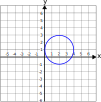
\includegraphics[width=0.6\textwidth]{circles_00.pdf}
\end{figure}


\rightline{ (Soluzione a pagina \pageref{circs_01} )}

\vspace{1cm}
\hrule
\vspace{1cm}

\item  \label{circ_02}

State the center and radius of the circle graphed below and construct the equation for it.

\begin{figure}[H]
\centering
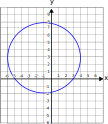
\includegraphics[width=0.6\textwidth]{circles_01.pdf}
\end{figure}


\rightline{ (Soluzione a pagina \pageref{circs_02} )}

\item  \label{circ_03}

State the center and radius of the circle described by the equation and graph it.

\begin{equation*}
\begin{split}
(a): (x-2)^2+(y+3)^2=9 \\
\\
(b): (x-2)^2+(y+5)^2=4 \\
\\
(c): (x+9)^2+y^2=25 \\
\\
(d): (x+\frac{1}{2})^2+(y-\frac{3}{5})^2=\frac{161}{100}
\end{split}
\end{equation*}


\rightline{ (Soluzione a pagina \pageref{circs_03} )}

\vspace{1cm}
\hrule
\vspace{1cm}


\item  \label{circ_04}

Find the center and radius of the circle 
\begin{equation*}
x^2+y^2-6x+8y+24=0 
\end{equation*}



\rightline{ (Soluzione a pagina \pageref{circs_04} )}

\vspace{1cm}
\hrule
\vspace{1cm}



\item  \label{geop_01}
% from savemyexams.com
A circle has equation 

\begin{equation*}
x^2+y^2+14x-6y=-41
\end{equation*}

The lines $l_1$ and $l_2$ are both tangents to the circle, 
and they intersect at the point $(0,14)$.

\begin{figure}[h]
\centering
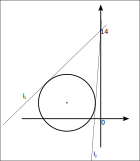
\includegraphics[width=0.4\textwidth]{01.pdf}
\end{figure}

Find the equatons of $l_1$ and $l_2$ giving your answers in the form $y=mx+c$.

( Soluzione a pagina \pageref{geos_01} )
% soluzione da qui: https://www.quora.com/A-circle-has-the-equation-x-2-6x-2y-y-2-7-The-lines-l1-and-l2-are-tangents-to-the-circle-they-intersect-at-R-0-6-How-do-you-find-the-equations-of-l1-and-l2


\vspace{1cm}
\hrule
\vspace{1cm}


\item  \label{circ_06}

Date le due circonferenze definite dalle seguenti equazioni:

\begin{equation*}
\begin{split}
(a): x^2+y^2-2x-4y-4=0 \\
\\
(b): x^2+y^2-4x-2y+4=0
\end{split}
\end{equation*}

Possiamo affermare che le due circonferenze:

\begin{itemize}
\item[A)] sono tangenti
\item[B)] sono disgiunte e la seconda è interna alla prima
\item[C)] si intersecano in due punti distinti
\item[D)] si intersecano in quattro punti distinti
\item[E)] sono disgiunte e la prima è interna alla seconda
\end{itemize}


\rightline{ (Soluzione a pagina \pageref{circs_06} )}

\vspace{1cm}
\hrule
\vspace{1cm}


%\item  \label{circ_07}
%\rightline{ (Soluzione a pagina \pageref{circs_07} )}
%
%\vspace{1cm}
%\hrule
%\vspace{1cm}
%
%
%\item  \label{circ_08}
%\rightline{ (Soluzione a pagina \pageref{circs_08} )}
%
%\vspace{1cm}
%\hrule
%\vspace{1cm}
%
%
%\item  \label{circ_09}
%\rightline{ (Soluzione a pagina \pageref{circs_09} )}
%
%\vspace{1cm}
%\hrule
%\vspace{1cm}
%
%
%\item  \label{circ_10}
%\rightline{ (Soluzione a pagina \pageref{circs_10} )}
%
%\vspace{1cm}
%\hrule
%\vspace{1cm}
%
%


\end{enumerate}

\pagebreak

